\documentclass[letterpaper]{article}

\setlength{\textheight}{8.875in}
\setlength{\topmargin}{0in}
\setlength{\headheight}{0in}

\usepackage{multirow}
\usepackage{float,graphicx}
\usepackage[breaklinks=true,hidelinks]{hyperref}
\appto\UrlBreaks{\do\-}

\begin{document}
\title{Paleo Oceanography Model Report}

\author{Ethan Chung\\
    {\tt\small University of Hawaii}\\
    {\tt\small ICS 637: Deep Learning with Neural Networks}\\
    {\tt\small [redacted]@hawaii.edu}}

\maketitle

\section{Introduction}

    This project applies image classification to identify single-celled organisms known as foraminifera (forams) from microscope images. These images are sourced from borehole samples taken from the Santa Barbara Basin, spanning an 800-year interval during the Common Era (1249–2008 CE) \cite{kahanamoku23}. The primary goal of this project is to classify the input images into one of 53 foraminifera species labels, with an additional label for "non-forams" classifications.

    Foraminifera play a crucial role in climate change as marine calcifiers. When foraminifera die, their shells, which are built up by calcium carbonate, sink to the ocean floor, neutralizing acidity and helping regulate atmospheric carbon dioxide over time. Rising CO2 levels and ocean acidification threaten foraminifera by causing stress, reducing metabolism, and impairing shell repair. This decreases calcification, weakening their ability to neutralize acidity, which results in an increase of ocean acidification, thereby disrupting the carbon cycle \cite{kerlin17}.
    
\section{Dataset}

    The dataset for this model is originally sourced from Kahanamoku et al. (2023); however, only a portion of the entire dataset is provided for the Kaggle competition. The dataset provided is pre-split into training and test sets, consisting of 8,653 and 2,174 images, respectively. The training set is further divided into an 80/20 split for training and validation. Each image in the training set is labeled with one of 53 foraminifera species, including an extra label to classify non-forams. The dataset is imbalanced, as shown in Figure \ref{fig:class_distribution}.
    
    The model is trained on the training set, while the validation set is used for learning rate adjustment and model selection. To evaluate the model, predictions are made on the test set, outputted to a file, and submitted to the Kaggle competition, where they are evaluated on public and private leaderboards to compute the corresponding zero-one loss (accuracy) scores.

    \begin{figure}[H]
        \centering
        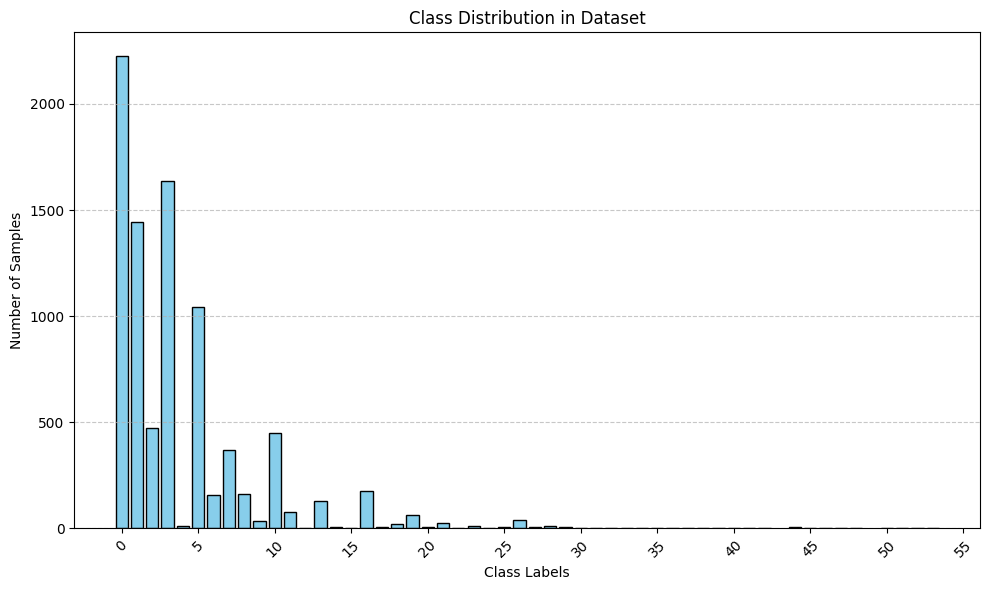
\includegraphics[width=1\linewidth]{Figure0-ClassDistribution.png}
        \caption{Most samples in the dataset are concentrated in a few classes, while many others have very few samples. All classes had at least one sample.}
        \label{fig:class_distribution}
    \end{figure}
    
\section{Model Architecture}

    Convolutional Neural Networks (CNNs) are well-suited for image classification by learning patterns like edges, textures, and shapes directly from image data. This project employs a pre-trained ResNet-50 model for transfer learning. The early layers of the pre-trained ResNet-50 are frozen to retain general features, while the last three layers are unfrozen for fine-tuning to learn specific features for foraminifera classification.

    This model is trained with mini-batch gradient descent with batch sizes of \texttt{100} for \texttt{2} iterations per epoch. The loss function being optimized is categorical cross-entropy loss. The optimization is performed using the AdamW optimizer, with a learning rate of \texttt{0.001} and weight decay of \texttt{1e-5}. The learning rate is dynamically adjusted using the ReduceLROnPlateau scheduler, which monitors the validation loss and reduces the learning rate by a factor of \texttt{0.5} if the validation loss does not improve for \texttt{2} consecutive epochs. Hyper-parameter values were chosen manually as sensible defaults, and no further hyper-parameter tuning was performed.
    
\section {Features \& Pre-processing}

    \subsection{Image Pre-processing}
        
        All images are rescaled to a resolution of \texttt{224x224} pixels, which aligns with the original input size of the images used to train the ResNet-50 model. Additionally, the image channels are normalized to a mean of \texttt{[0.5, 0.5, 0.5]} and a standard deviation of \texttt{[0.225, 0.225, 0.225]}. 

    \subsection{Data Augmentation}
        
        As the dataset is rather small, data augmentation is used to increase diversity by generating modified variants transformed by translation, rotation, contrast, inversion, etc. The following auto-augmentation methods are tested:

        \begin{itemize}
            \item AutoAugment: Applies augmentations based on learned policies, which specify the probability of applying a particular augmentation and the magnitude of applying that augmentation.
            
            \begin{figure}[H]
                \centering
                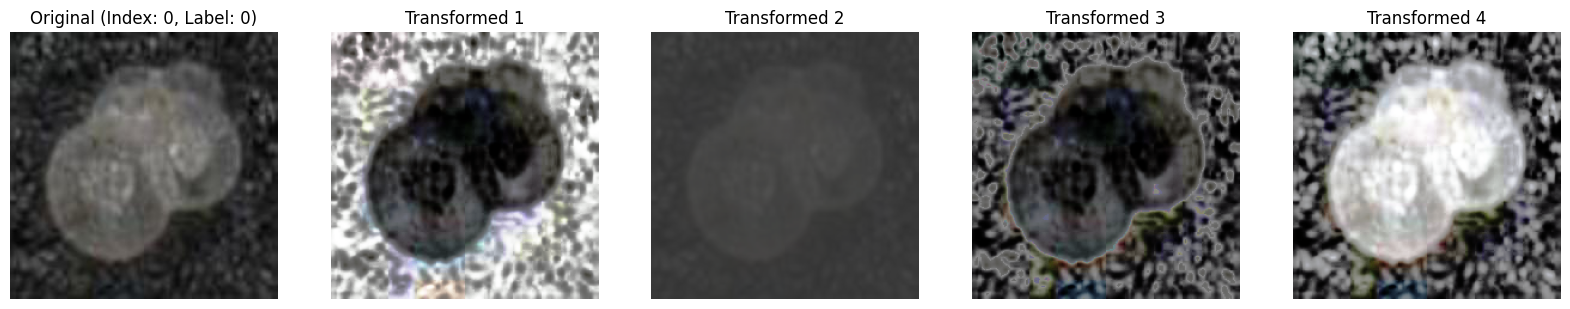
\includegraphics[width=1\linewidth]{Figure1-AutoAug.png}
                \caption{AutoAugment sample augmentations}
                \label{fig:autoaug}
            \end{figure}
            
            \item RandAugment: Randomly selects augmentations from a predefined set of transformations, applying them with uniform probability.

            \begin{figure}[H]
                \centering
                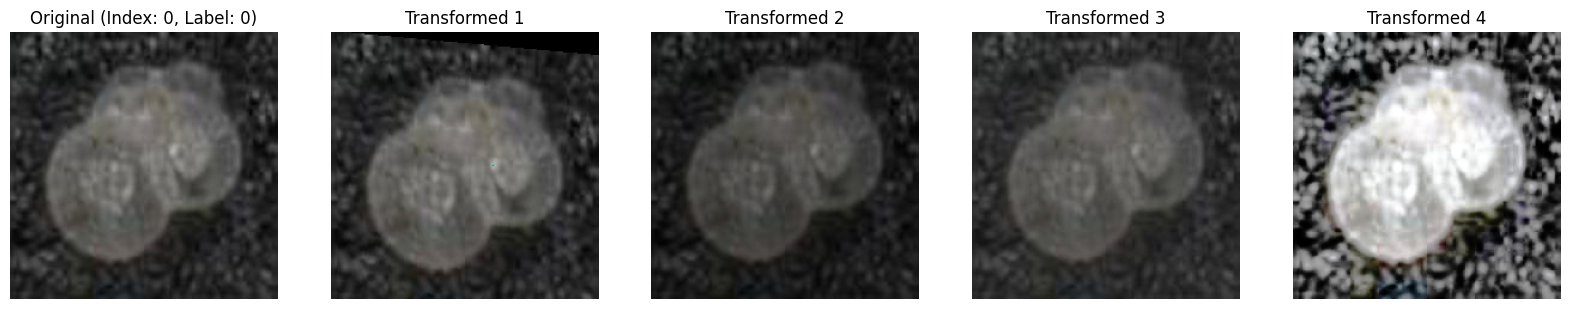
\includegraphics[width=1\linewidth]{Figure2-RandAug.png}
                \caption{RandAugment sample augmentations}
                \label{fig:randaug}
            \end{figure}
            
            \item TrivialAugmentWide: Applies a single augmentation per image, with the transformation randomly selected for each image.

            \begin{figure}[H]
                \centering
                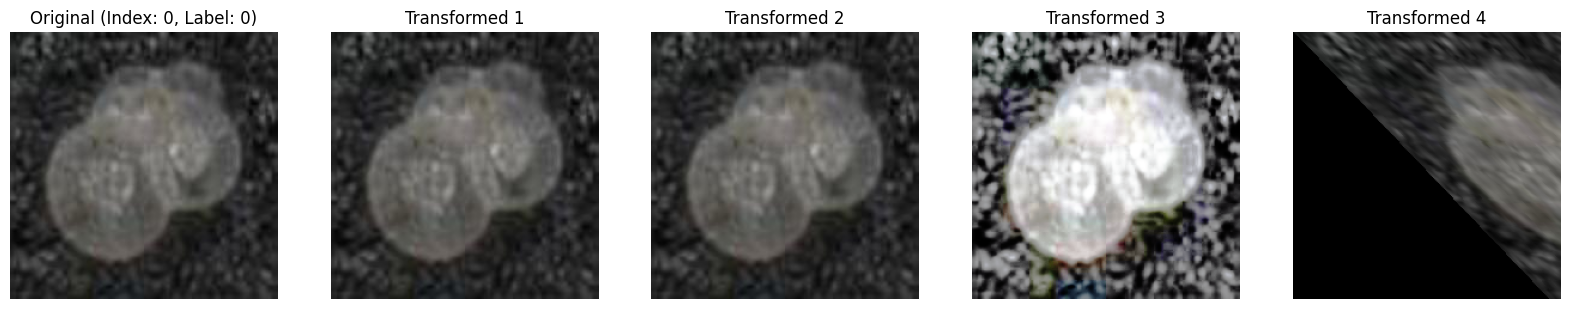
\includegraphics[width=1\linewidth]{Figure3-TAW.png}
                \caption{TrivialAugmentWide sample augmentations}
                \label{fig:taw}
            \end{figure}
            
            \item AugMix: Combines multiple augmentations to maintain semantic similarity while introducing variability.

            \begin{figure}[H]
                \centering
                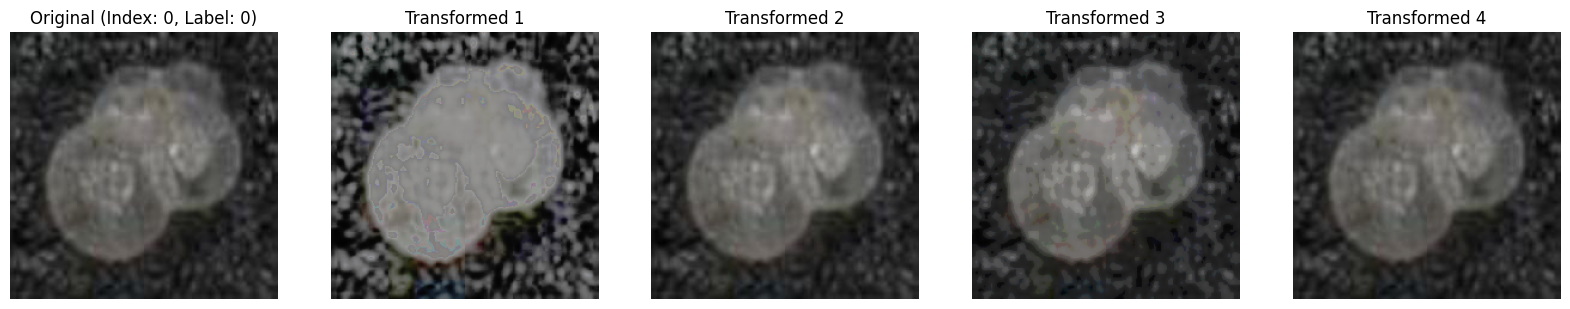
\includegraphics[width=1\linewidth]{Figure4-AugMix.png}
                \caption{AugMix sample augmentations}
                \label{fig:augmix}
            \end{figure}
        \end{itemize}

\section{Results}

    The classification model's performance was assessed using \textbf{zero-one loss (accuracy)} on the validation set during training and on a held-out test set. The predictions obtained from evaluating the model on the test set are then submitted to the Kaggle competition, where two held-out public and private leaderboard sets are evaluated using the predictions from the test set to obtain an accuracy score. Table \ref{tab:model_accuracies} summarizes the results for the various auto augmentation strategies utilized.
    
    The baseline model (without augmentation) achieved the highest validation accuracy of 84.70\%, matched only by the AugMix method. However, AugMix underperformed on the public and private leaderboards, scoring 81.36\% and 81.01\%, respectively. RandAugment demonstrated strong performance across all metrics, with validation accuracy reaching 84.20\% and leaderboard scores of 82.73\% (public) and 83.61\% (private), making it the most balanced method.

    AutoAugment and TrivialAugmentWide displayed slightly lower validation accuracies of 81.90\% and 83.20\%, respectively. AutoAugment showed consistent performance across metrics, with a marginal -0.08\% decrease in the public leaderboard and a +0.78\% improvement in the private leaderboard compared to its validation accuracy. TrivialAugmentWide achieved moderate results on the validation set, but experienced significant drops in accuracy on both leaderboards, with -3.20\% (public) and -1.17\% (private).

    While AutoAugment demonstrated consistent performance across metrics, suggesting minimal overfitting on the training dataset, RandAugment ultimately yielded the best overall results on both the public and private leaderboards.
    
    \begin{table*}[h!]
        \centering
        \caption{Model Accuracies Using Different Auto-Augmentation Techniques}
        \resizebox{\textwidth}{!}{%
        \begin{tabular}{||l|c|c|c||} 
            \hline
            \multicolumn{1}{||c|}{\textbf{Augmentation}} & \multicolumn{1}{c|}{\textbf{Best Validation}} & \multicolumn{1}{c|}{\textbf{Public}} & \multicolumn{1}{c||}{\textbf{Private}} \\
            \multicolumn{1}{||c|}{\textbf{Method}}      & \multicolumn{1}{c|}{\textbf{Accuracy (\%)}} & \multicolumn{1}{c|}{\textbf{Accuracy (\%)}} & \multicolumn{1}{c||}{\textbf{Accuracy (\%)}} \\
            \hline\hline
            None (Baseline)           & \textbf{84.70} & 81.36 & 82.87 \\ 
            AutoAugment               & 81.90 & 81.82 & 82.68 \\ 
            RandAugment               & 84.20 & \textbf{82.73} & \textbf{83.61} \\ 
            TrivialAugmentWide        & 83.20 & 80.00 & 82.03 \\ 
            AugMix                    & \textbf{84.70} & 81.36 & 81.01 \\ 
            \hline
        \end{tabular}%
        }
        \label{tab:model_accuracies}
    \end{table*}

\section{Conclusion}

    Among the five models trained, the model using RandAugment achieved the best zero-one loss (accuracy) on both the public and private leaderboards, with 82.73\% and 83.61\% accuracy, respectively. However, a likely discrepancy between the training and test datasets is that the training set may be more skewed toward certain labels compared to the test set. This imbalance can limit the model's ability to generalize to unseen data. More training data alongside a more balanced dataset could improve both the model's performance and generalization.

    Although hyper-parameter tuning was manually performed by testing various auto-augmentation techniques, hyper-parameter tuning was not conducted on parameters like the learning rate or weight decay for the AdamW optimizer. Using a method like GridSearchCV to explore the hyper-parameter search space could yield better performance on the public and private leaderboards. In addition, incorporating evaluation metrics other than accuracy may better represent the model’s effectiveness. Yuan et al. (2015) suggests that the Average Precision (AP) metric, derived from the area under the Precision-Recall (PR) curve, provides a more representative measure of performance in cases of highly imbalanced datasets \cite{yuan15}.

\section{Data Availability}
    The original dataset can be sourced from Kahanamoku et al. (2023) \cite{kahanamoku23}, while the adapted dataset used for this project can be found from the Kaggle competition at \url{https://www.kaggle.com/competitions/Paleo-Oceanography}.

\section{Code Availability}
    All code for this report is available at \url{https://github.com/echung32/ics637-paleo-oceanography}.

\begin{thebibliography}{9}
    \bibitem{kahanamoku23}
    Kahanamoku, S., Samuels-Fair, M., Kamel, S. M., Stewart, D., Kahn, L., Titcomb, M., Mei, Y. A., Bridge, R. C., Li, Y. S., Sinco, C., Epino, J. T., Gonzalez-Marin, G., Latt, C., Fergus, H., \& Finnegan, S. (2023). Twenty-two thousand Common Era benthic foraminifera from the Santa Barbara Basin [Data set]. Zenodo. \url{https://doi.org/10.5281/zenodo.10067274}
    
    \bibitem{kerlin17}
    Kerlin, K. E. (2017). Tiny Shells Indicate Big Changes to Global Carbon Cycle. UC Davis. \url{https://www.ucdavis.edu/news/tiny-shells-indicate-big-changes-global-carbon-cycle}

    \bibitem{yuan15}
    Yuan, Y., Su, W., \& Zhu, M. (2015). Threshold-free measures for assessing the performance of medical screening tests. Frontiers in public health, 3, 57. \url{https://doi.org/10.3389/fpubh.2015.00057}

\end{thebibliography}

\end{document}
